
\section{Basic Coq constructions} \label{sec2}

We will now introduce some basic constructions in Coq and their
corresponding homotopy theoretic interpretations.  We mention here
that there is an accompanying Coq file which includes all of the Coq
code discussed here, as well as some additional code.\footnote{The
  Coq file can be found either as supplementary data attached to the
  arXiv version of this paper or on the second author's webpage.}

\subsection{The Coq proof assistant} \label{Coq}

The Coq proof assistant \cite{Coq,Bertot:2004uj,Chlipala:CP} is a
computer system which is based one flavor of Martin-L\"of type theory
called the \emph{calculus of inductive constructions} and based in
part on the earlier \emph{calculus of constructions}
\cite{Coquand:1988eq} due to Coquand and Huet. 

In February 2010 Voevodsky \cite{Vo2012a} began writing a Coq library
of formalized mathematics based on the univalent model.  The resulting
library can currently be found online at the following location:
\begin{center}
\url{http://github.com/vladimirias/Foundations/}. 
\end{center}
There is also an HTML version of the library which can be found at Voevodsky's web page
\begin{center}
\url{http://www.math.ias.edu/~vladimir}
\end{center}
In addition to Voevodsky's library, there is also a repository which
is being developed by other researchers in homotopy type theory which
can be found at
\begin{center}
  \url{http://github.com/HoTT/HoTT}
\end{center}
Documentation on how to configure Coq for each of these libraries can
be found on the respective websites.  We expect a unification of these
libraries to occur at some point during the Special Year being held at
the Institute for Advanced Study during the 2012 - 2013 academic year.
For now though we work mostly in the style of Voevodsky's library.

While we will not explain here how to install or process a Coq file,
it is nonetheless worth mentioning that the way a Coq file is
generally processed is in an \emph{active} manner.  That is, one
processes the file in a step-by-step way and as one does so Coq
provides feedback regarding the current state of the file.
\begin{figure}[H]
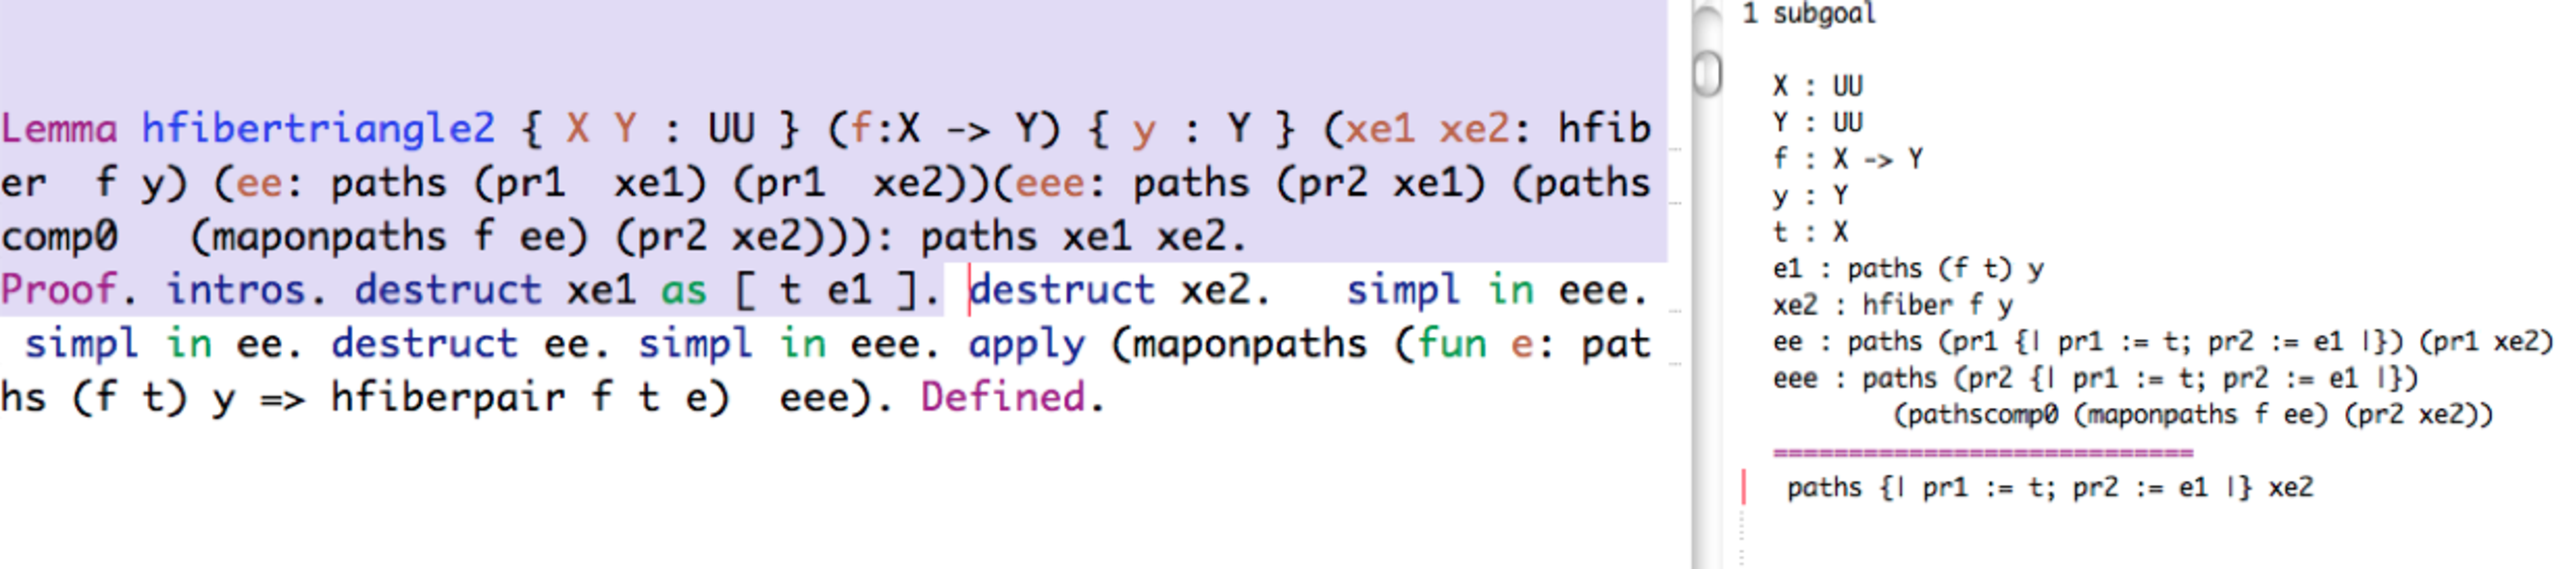
\includegraphics[width=4.9in]{screen}
  \caption{A screen with separate compartments when working with
    Coq. The code entered by the user is here displayed in the left
    compartment. The next goal required by Coq in order to complete
    the currently active proof appears in the upper right compartment.}
  \label{fig:diffeo}
\end{figure}
For example, Figure \ref{fig:diffeo} illustrates a Coq file currently
being processed.  The user is currently in the middle of processing a
proof (indicated in the left-hand pane of the image) and the shaded
text denotes the part of the file which has so far been processed by
Coq.  The right-hand pane is one of two mechanisms which Coq has for
providing the user with feedback.  In particular, this pane indicates
the current state of the proof which is being carried out.  Thus, as
the user progresses through a proof the output changes so as to always
indicate what remains to be done in order to complete the proof.
Further, more detailed, examples of this process are given below.

\subsection{Types and terms in Coq}\label{sec:sentences}

The Coq proof assistant, being based as it is on a form of type
theory, allows us to formalize and verify reasoning about types and
terms.  Throughout our discussion, the reader should have in mind the
interpretation of type theory described in Section
\ref{sec:homotopy_interp}.  Coq comes with a number of types and
type forming operations already built-in.  Using these it is possible
to define new types.  The first thing we want to do is to select a
fixed universe of small types with which we will work.  This is
accomplished by the following code:
\begin{center}
  \begin{coqcode}
Definition UU := Type.
  \end{coqcode}
\end{center}
Here the expression \verb|Type| is a built-in type in the Coq
system which is a universe of types (in a suitable technical sense).
The definition above then serves to define \verb|UU| to be this
fixed built-in universe of types.  We think of the terms of type
\verb|UU| as the small spaces and the universe \verb|UU|
itself as the (large) space of small spaces.
Mathematically this is roughly the same as fixing a Grothendieck
universe and letting \verb|UU| be the corresponding space of
spaces in the universe.  

The main reason for doing this, aside from notational convenience, is
a technical one arising from the internal
mechanism of Coq.  Namely, Coq secretly assigns indices to each
occurrence of \verb|Type| in a way which ensures a consistent
indexing.  However, we would like to work with one fixed universe and
not with an entire hierarchy thereof, and this is accomplished by
adopting the definition above.\footnote{If you would like to see the
  explicit indexing of universes, then you can add the line
  {\texttt{Set Printing Universes.}} to your Coq file.}  
The type \verb|UU| corresponds to $\UU$ from Section
\ref{sec:univalent_model} above.  Henceforth, any
statement of the form \verb|A : UU| should be thought of as
asserting that $A$ is a small space.

One interesting feature of the Coq system is that types are themselves
terms.  In particular, the ``type'' \verb|UU| above is itself a term of type \verb|Type|, where
this latter \verb|Type| is given the index $(n+1)$ when
\verb|UU| has index $n$. That is, being a type is really the same as being
a term in a higher universe.

\subsection{A direct definition involving function spaces}\label{sec:direct_def}

In order to illustrate some further features of the Coq system, we
will define some basic construction on function spaces.  First, we
define, for any small type, the identity function:
\begin{center}
  \begin{coqcode}
Definition idfun ( A : UU ) : A -> A := fun x => x.
  \end{coqcode}
\end{center}
Let us dissect this line of code and try to understand each of the
ingredients.  A definition, such as this one, is what we will call a
\emph{direct definition} and such a definition has the abstract form
summarized (together with the two examples we have so far encountered)
in Figure \ref{fig:direct}.
\begin{figure}[H]
  \centering
  \begin{tabular}{cccccccc}
    \verb|Definition| & \emph{name} &
    \emph{parameters} & : & \emph{type} & := &
    \emph{explicit definition} & .\\
    \hline
    & \verb|UU| & & & & & \verb|Type| &\\
    & \verb|idfun| & \verb|( A : UU )| &  &
    \verb| A -> A | & & \verb|fun x => x| &
  \end{tabular}
  \caption{Direct definitions in Coq.}
  \label{fig:direct}
\end{figure}

Several remarks about Figure \ref{fig:direct} are in order.  First, the \emph{name} is the name
given to the term.  This can be whatever (modulo some restrictions on
the syntactic form) the user likes.  The \emph{type} is the type of
the term being defined.  I.e., we have that \emph{name} is of type
\emph{type}.  The next thing to note is that the \emph{parameters} can
be a list of terms variables of fixed types.  In the case of
\verb|idfun| there is just a single parameter: the type
\verb|A : UU|; in the case of \verb|UU| there are no
parameters at all.  Within a definition, the parameters should be
enclosed in brackets as in \verb|( A : UU )|.  Next, note that
it is not strictly necessary to declare the type.  When no type is
given, Coq will infer the type.  Finally, note that the period at the
end of the definition must be included in order for Coq to correctly
parse the input.

Coming back to the definition of \verb|idfun|, it is worth
mentioning that the type \verb|A -> A| is the way of denoting the
function space $A^{A}$ in Coq.  That is, for types \verb|A| and
\verb|B|, the type \verb|A -> B| is the type of functions
from \verb|A| to \verb|B|.  For us, this type should be
thought of more specifically as the type of all continuous functions
from the space \verb|A| to the space \verb|B|.  The
remaining part of this definition is the actual content of the
definition: \verb|fun x => x|.  In this definition, the
expressions \verb|fun| and \verb|=>| go together and tell us
that it is the function which takes a point $x$ in $A$ and gives back $x$.
That is, \verb|fun ... => ...| is the same as giving a definition
of a function by writing $\ldots\mapsto\ldots$ or (for those familiar
with lambda calculus) using lambda abstraction.  In particular, the
definition states that \verb|idfun| is the function given by
$x\mapsto x$ (i.e., $\lambda_{x}.x$).

We can now play around a bit with the type checking mechanisms of
Coq.  Let us enter the following into the Coq code:
\begin{center}
  \begin{coqcode}
Section idfun_test.    
Variable A : UU.
Variable a : A.
  \end{coqcode}
\end{center}
The first line tells Coq that we are starting a new section of the
file in which we will introduce certain hypotheses.  The next line
tells Coq that we would like to assume, for the duration of the
current section, that \verb|A| is a space in \verb|UU|.  The
final line similarly tells Coq that we are assuming given a point
\verb|a| of \verb|A|.  Now, if we add the following line to
our Coq file and process up to this point, we will be able to see what
type the term \verb|idfun A| has:
\begin{center}
  \begin{coqcode}
Check idfun A.
  \end{coqcode}
\end{center}
Coq will respond by telling us 
\begin{center}
  \begin{coqcode}
idfun A : A -> A.
  \end{coqcode}
\end{center}
Similarly, if we enter
\begin{center}
  \begin{coqcode}
Check idfun _ a.
  \end{coqcode}
\end{center}
Then Coq replies with \verb|idfun A a : A|.  Here note that we
write \verb|idfun _ a| to tell Coq that we would like for it to
guess the parameter (in this case \verb|A|) which should go
in the place indicated by the underscore.  Finally, we close the
section by entering
\begin{center}
  \begin{coqcode}
End idfun_test.
  \end{coqcode}
\end{center}
After entering this line of code, the variables \verb|A| and
\verb|a| are no longer declared.\footnote{You can verify this by
  trying \texttt{Check A.} and observing the response from Coq.
  Be sure to remove this line from your code though otherwise you
  won't be able to go any further!}

\subsection{An indirect definition involving function spaces}

We will now show, given functions $f:A\to B$ and $g:B\to C$, how to
construct the composite $g\circ f : A \to C$ type theoretically.  In
order to introduce \emph{indirect} definitions, we will give two
ways to construct $g\circ f$.

The utility of indirect definitions in Coq is that sometimes it is not
easy to see how to give the explicit definition of a term.  This is
especially true as one starts working with increasingly complicated
definitions.  As such, rather than having to struggle to define
exactly the required term it is possible to construct the term being
defined as a kind of proof.  Along the way, as this proof is
constructed, certain automation possible in Coq can be employed.  In
order to see how this works in practice, let us introduce our first
indirect definition.
\begin{center}
  \begin{coqcode}[frame=single,backgroundcolor=\color{mylight},framerule=0pt]
Definition funcomp_indirect ( A B C : UU ) ( f : A -> B ) ( g : B -> C ) : A -> C.
Proof.
  intros x. apply g. apply f. assumption.
Defined.
  \end{coqcode}
\end{center}
The first observation about this definition is that it looks like
everything to the left of the \verb|:=| in a direct definition.
In this case there are three parameters of type \verb|UU|
(namely, \verb|A|, \verb|B| and \verb|C|).  There is
also one parameter of type \verb|A -> B| (namely,
\verb|f|).  Finally, there is one parameter of type \verb|B -> C| (namely, \verb|g|).  

After the first full stop of an indirect definition, we encounter the
start of the proof.  This is given by the line
\begin{center}
  \begin{coqcode}
Proof.
  \end{coqcode}
\end{center}
Likewise, the end of the proof is indicated by 
\begin{center}
  \begin{coqcode}
Defined.
  \end{coqcode}
\end{center}
Between the start of the proof and the end of the proof is a sequence
of what are called \emph{tactics}, which allow one to construct, using
the given parameters, the required term.  One limitation of writing an
article which includes proofs in Coq, is that proofs in Coq are
usually constructed using ``backward'' reasoning and so it can be hard to
read for the uninitiated.  In particular, the nature of Coq is such
that, \emph{qua} interactive proof assistant, proofs can be understood
better by directly watching the output of a Coq session, where an
additional window appears after each step, giving us precise
explanations on any given step of the proof.  We have included in
Figure \ref{figure:indirect_funcomp} the output from Coq as we move
through the proof of \verb|funcomp_indirect|.  Readers
should not be discouraged if they are unable to read Coq proofs
directly: it is much easier if you are going through the proofs yourself in the
computer.

\begin{figure}[H]
  \begin{tikzpicture}
    \node[smallcoqbox] (zero)  at (0,0) {%
      \begin{minipage}{4.25cm}
        \footnotesize
        
        \vphantom{\texttt{x : A}}
        
        \noindent\verb|A : UU|
        
        \noindent\verb|B : UU|
        
        \noindent\verb|C : UU|
        
        \noindent\verb|f : A -> B|
        
        \noindent\verb|g : B -> C|
        
        \noindent\verb|============================|
        
        \noindent\verb| A -> C|
      \end{minipage}
    };
    \node[anchor=north east, inner sep=2pt] (titlezero) at
    (zero.north east) {\emph{Start of proof}};
    \node[smallcoqbox] (one) at (5.25,0) {%
      \begin{minipage}{4.25cm}
        \footnotesize
        \noindent\verb|A : UU|
        
        \noindent\verb|B : UU|
        
        \noindent\verb|C : UU|
        
        \noindent\verb|f : A -> B|
        
        \noindent\verb|g : B -> C|
        
        \noindent\verb|x : A|
        
        \noindent\verb|============================|
        
        \noindent\verb| C|
      \end{minipage}
    };
    \node[anchor=north east, inner sep=2pt] (titleone) at
    (one.north east) {\emph{after} \verb|intros x.|};
    \node[smallcoqbox] (two) at (0,-4.25) {%
      \begin{minipage}{4.25cm}
        \footnotesize
        \noindent\verb|A : UU|
        
        \noindent\verb|B : UU|
        
        \noindent\verb|C : UU|
        
        \noindent\verb|f : A -> B|
        
        \noindent\verb|g : B -> C|
        
        \noindent\verb|x : A|
        
        \noindent\verb|============================|
        
        \noindent\verb| B|
      \end{minipage}
    };
    \node[anchor=north east, inner sep=2pt] (titletwo) at
    (two.north east) {\emph{after} \verb|apply g.|};
    \node[smallcoqbox] (three) at (5.25,-4.25) {%
      \begin{minipage}{4.25cm}
        \footnotesize
        \noindent\verb|A : UU|
        
        \noindent\verb|B : UU|
        
        \noindent\verb|C : UU|
        
        \noindent\verb|f : A -> B|
        
        \noindent\verb|g : B -> C|
        
        \noindent\verb|x : A|
        
        \noindent\verb|============================|
        
        \noindent\verb| A|
      \end{minipage}
    };
    \node[anchor=north east, inner sep=2pt] (titlethree) at
    (three.north east) {\emph{after} \verb|apply f.|};
  \end{tikzpicture}
  \caption{Coq output during indirect definition of function
    composition.}
  \label{figure:indirect_funcomp}
\end{figure}

We will now go through the proof one step at a time.  Notice that once the proof is started Coq
displays the hypotheses (above the line \verb|=======|) together
with the current goal (below the line).  Since the goal is to
construct a function \verb|A -> C| we are allowed to assume given an
arbitrary term \verb|x : A|.  This is accomplished in Coq by
entering \verb|intros x|.  Note that the name \verb|x| here
is something which we have chosen and the user can choose this name
freely (or it can be omitted, in which case the Coq system will supply
a name of its own choosing).  As such, after processing
\verb|intros x|, the output has changed (as indicated in Figure
\ref{figure:indirect_funcomp}) by adding a new hypothesis 
(\verb|x : A|) and changing the goal to \verb|C|.  This means that we now
need to supply a term of type \verb|C|.  To accomplish this, we
note that we are given a function \verb|g : B -> C| and so it
suffices to supply a term of type \verb|B|.  We communicate the
fact that we intend to use \verb|g| to obtain the goal by
entering \verb|apply g|.  The effect of this is to change the
goal from \verb|C| to \verb|B| since \verb|B| is the
domain of \verb|g|.  Applying the same reasoning now with
\verb|f| we are in the final situation indicated in Figure
\ref{figure:indirect_funcomp}.  Because we have as a hypothesis the term
\verb|x : A| and the current goal is to construct a term of type
\verb|A| we may simply communicate to the Coq system that
there is already a term of the required type appearing among the
hypotheses.  This is accomplished by entering \verb|assumption|.
Indeed, at this point, Coq tells us
\begin{center}
  \begin{coqcode}
No more subgoals.
  \end{coqcode}
\end{center}
and the proof is complete.  Note that we \emph{must} add the final
``\verb|Defined.|'' in order for the Coq system to correctly
record the proof.

We now turn to the corresponding direct definition:
\begin{center}
  \begin{coqcode}
Definition funcomp { A B C : UU } ( f : A -> B ) ( g : B -> C ) := fun x : A => g ( f x ).
  \end{coqcode}
\end{center}
One thing worth noting about this definition is that here we have
enclosed the first three parameters in curved brackets as \verb|{A B C : UU}| in order to indicate to the Coq system that these
parameters are \emph{implicit}.  Implicit parameters do not need to be
supplied (when the term is applied) by the user and the system will
try to infer the values of these parameters.  In this case, these can
be inferred from the types of \verb|f| and \verb|g|.  Note
also that we have here not given explicitly the type of the term being
defined.  As such, we must include the additional typing data
\verb|x : A| in the definition in order for the Coq system to be
able to infer the type of the term. 

We can now check that our definition agrees with the direct
one by entering:
\begin{center}
  \begin{coqcode}
Print funcomp.
Print funcomp_indirect.
  \end{coqcode}
\end{center}
The effect of \verb|Print| is to output both the type and
explicit definition of the term in question.  In particular, even if
the term in question was defined indirectly, as our
\verb|funcomp_indirect| was, it is an \emph{explicit term
as far as Coq is concerned}, and when \verb|Print| is used Coq
will unfold the term to give a completely explicit description.

To understand what this means, simply think of a linear differential
equation for which it is possible to explicitly write down
the solutions. The solution set can be difficult to write down, but it can
be done. Although you may not want to have these solutions in front of
you, you know that the explicit solutions are available if they are required (say, to
verify that they satisfy a certain equation).  The Coq system
effectively keeps track of this kind of book-keeping for the user.
